
\section{Details on Bracha-layer Byzantine behavior\label{anx:detail_bracha_layer_attack}}



Because Bracha's Byzantine Reliable Broadcast algorithm \cite{asynchronous_byzantine_agreement_protocols} relies on collecting (and thus waiting for) a certain number of ECHO and READY messages from other nodes, the adversary can statistically delay this $\mathtt{rdlver}$ operation on all nodes via infecting a minority of nodes.
In this scenario, infected nodes will not emit ECHO and READY messages for vertices that contain transactions from the target client.

Let us indeed suppose that the probability to receive an emitted ECHO before timestamp $z$ is given by variable $X$.
Among $n$ trials, the probability of having collected exactly $k \leq n$ such messages before $z$ is:
\[
\binom{n}{k} * X^k * (1-X)^{n - k}
\]

For vertices that contain transactions from the target client, sabotaged nodes never send these ECHO messages (we always have $X=0$ for any timestamp $z$) and can therefore be ignored when counting the numbers of messages.
Therefore, given $b \leq f$ the number of sabotaged nodes, the probability of having collected at least $\lfloor \frac{n+f}{2} \rfloor + 1$ ECHO messages from distinct nodes before $z$ is:
\[
Y = \sum_{k = \lfloor \frac{n+f}{2} \rfloor + 1}^{n-b} \binom{n - b}{k} * X^k * (1-X)^{n - b - k}
\]


$\mathtt{rdlver}$ then requires collecting at least $2*f+1$ READY messages, which probability we can approximate as follows:
\[
Z = \sum_{k = 2*f + 1}^{n-b} \binom{n - b}{k} * Y^k * (1-Y)^{n - b - k}
\]



\begin{figure}[h!]
\vspace*{-.25cm}
    \centering

\scalebox{.85}{
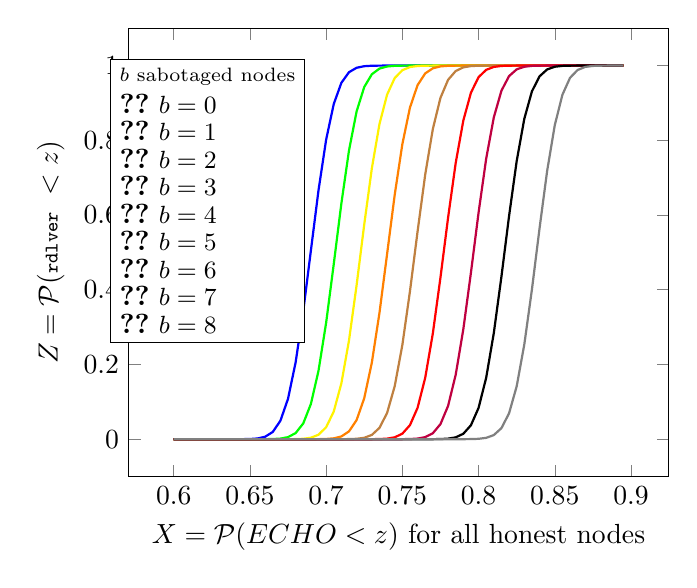
\begin{tikzpicture}
\begin{axis}[ 
    xlabel={$X = \mathcal{P}(ECHO < z)$ for all honest nodes},
    ylabel={$Z = \mathcal{P}({\scriptstyle\mathtt{rdlver}} ~ < z)$},
    ylabel near ticks,
]
  
\addplot[blue,thick] coordinates {
(0.6,7.381302483201029e-14)(0.605,1.4274422092481772e-12)(0.61,2.3640287899482728e-11)(0.615,3.35061485269394e-10)(0.62,4.061641311391178e-09)(0.625,4.208626703361768e-08)(0.63,3.725956277975355e-07)(0.635,2.817375392430534e-06)(0.64,1.819216568829287e-05)(0.645,0.00010031697704821041)(0.65,0.000472559322382775)(0.655,0.001902981482004006)(0.66,0.006558873825995439)(0.665,0.019384221346348204)(0.67,0.04925907210538647)(0.675,0.10805842114372206)(0.68,0.20577025217545059)(0.685,0.34277194314457987)(0.6900000000000001,0.5047380074491797)(0.6950000000000001,0.6660903979596449)(0.7000000000000001,0.8014634127933268)(0.7050000000000001,0.8970645337147377)(0.7100000000000001,0.9538649754638273)(0.7150000000000001,0.9822437643853553)(0.7200000000000001,0.9941614798069274)(0.7250000000000001,0.9983663805059899)(0.7300000000000001,0.9996122864190198)(0.7350000000000001,0.9999221521059732)(0.7400000000000001,0.9999868055607156)(0.7450000000000001,0.9999981159958161)(0.7500000000000001,0.9999997737892442)(0.7550000000000001,0.9999999772023577)(0.7600000000000001,0.9999999980751855)(0.7650000000000001,0.9999999998641301)(0.7700000000000001,0.9999999999919996)(0.7750000000000001,0.999999999999608)(0.7800000000000001,0.999999999999984)(0.7850000000000001,0.9999999999999996)(0.7900000000000001,0.9999999999999999)(0.7950000000000002,1.0)(0.8000000000000002,1.0)(0.8050000000000002,1.0)(0.8100000000000002,1.0)(0.8150000000000002,1.0)(0.8200000000000002,1.0)(0.8250000000000002,1.0)(0.8300000000000002,1.0)(0.8350000000000002,1.0)(0.8400000000000002,1.0)(0.8450000000000002,1.0)(0.8500000000000002,1.0)(0.8550000000000002,1.0)(0.8600000000000002,1.0)(0.8650000000000002,1.0)(0.8700000000000002,1.0)(0.8750000000000002,1.0)(0.8800000000000002,1.0)(0.8850000000000002,1.0)(0.8900000000000002,1.0)(0.8950000000000002,1.0)
};\label{b0}
\addplot[green,thick] coordinates {
(0.6,4.490759699730653e-18)(0.605,1.3091256482147663e-16)(0.61,3.290755956088118e-15)(0.615,7.127511475451589e-14)(0.62,1.3291666237089564e-12)(0.625,2.1325235805669003e-11)(0.63,2.94146667413955e-10)(0.635,3.4856945936756715e-09)(0.64,3.5464644692661476e-08)(0.645,3.0963145614907244e-07)(0.65,2.3187285343546966e-06)(0.655,1.4889789783934367e-05)(0.66,8.198353662527215e-05)(0.665,0.000387118564055316)(0.67,0.001568449722394253)(0.675,0.005458016675069293)(0.68,0.01633914126212621)(0.685,0.042179364351342286)(0.6900000000000001,0.09422580811501184)(0.6950000000000001,0.1830634404571597)(0.7000000000000001,0.31146488222125285)(0.7050000000000001,0.4684950693341753)(0.7100000000000001,0.6308731067656775)(0.7150000000000001,0.7727492647193246)(0.7200000000000001,0.8774263865080018)(0.7250000000000001,0.9426026580398292)(0.7300000000000001,0.976829559971615)(0.7350000000000001,0.9919803924137852)(0.7400000000000001,0.9976303699655735)(0.7450000000000001,0.9994043216190583)(0.7500000000000001,0.9998729726115105)(0.7550000000000001,0.9999770776533079)(0.7600000000000001,0.9999965075989335)(0.7650000000000001,0.99999955169857)(0.7700000000000001,0.9999999516186366)(0.7750000000000001,0.9999999956198408)(0.7800000000000001,0.9999999996681297)(0.7850000000000001,0.9999999999790126)(0.7900000000000001,0.9999999999988956)(0.7950000000000002,0.9999999999999518)(0.8000000000000002,0.9999999999999982)(0.8050000000000002,1.0)(0.8100000000000002,1.0)(0.8150000000000002,1.0)(0.8200000000000002,1.0)(0.8250000000000002,1.0)(0.8300000000000002,1.0)(0.8350000000000002,1.0)(0.8400000000000002,1.0)(0.8450000000000002,1.0)(0.8500000000000002,1.0)(0.8550000000000002,1.0)(0.8600000000000002,1.0)(0.8650000000000002,1.0)(0.8700000000000002,1.0)(0.8750000000000002,1.0)(0.8800000000000002,1.0)(0.8850000000000002,1.0)(0.8900000000000002,1.0)(0.8950000000000002,1.0)
};\label{b1}
\addplot[yellow,thick] coordinates {
(0.6,5.552137285219799e-23)(0.605,2.4142287054306263e-21)(0.61,9.114704900562854e-20)(0.615,2.9856993595941135e-18)(0.62,8.479363913991896e-17)(0.625,2.086190770918722e-15)(0.63,4.442914488445941e-14)(0.635,8.183696485892055e-13)(0.64,1.3026970678664695e-11)(0.645,1.7906098477952826e-10)(0.65,2.123669760957271e-09)(0.655,2.171642123200288e-08)(0.66,1.9134773676931015e-07)(0.665,1.4519593771410716e-06)(0.67,9.484239018891177e-06)(0.675,5.3316984276801864e-05)(0.68,0.00025795474251028976)(0.685,0.0010744090390422674)(0.6900000000000001,0.003855259085448833)(0.6950000000000001,0.011932704018399812)(0.7000000000000001,0.03192140293584917)(0.7050000000000001,0.07402178338990954)(0.7100000000000001,0.14942155213264618)(0.7150000000000001,0.2641426852825466)(0.7200000000000001,0.4123019911599361)(0.7250000000000001,0.5745819231262596)(0.7300000000000001,0.725209411120839)(0.7350000000000001,0.8435990672391458)(0.7400000000000001,0.9223346522463106)(0.7450000000000001,0.9666099537785198)(0.7500000000000001,0.9876464649445758)(0.7550000000000001,0.9960855104373783)(0.7600000000000001,0.998941756361155)(0.7650000000000001,0.9997567154107597)(0.7700000000000001,0.9999525717389982)(0.7750000000000001,0.9999921794128486)(0.7800000000000001,0.9999989119290262)(0.7850000000000001,0.9999998725837225)(0.7900000000000001,0.9999999874735761)(0.7950000000000002,0.9999999989690105)(0.8000000000000002,0.9999999999291795)(0.8050000000000002,0.9999999999959541)(0.8100000000000002,0.9999999999998085)(0.8150000000000002,0.9999999999999926)(0.8200000000000002,0.9999999999999998)(0.8250000000000002,1.0)(0.8300000000000002,1.0)(0.8350000000000002,1.0)(0.8400000000000002,1.0)(0.8450000000000002,1.0)(0.8500000000000002,1.0)(0.8550000000000002,1.0)(0.8600000000000002,1.0)(0.8650000000000002,1.0)(0.8700000000000002,1.0)(0.8750000000000002,1.0)(0.8800000000000002,1.0)(0.8850000000000002,1.0)(0.8900000000000002,1.0)(0.8950000000000002,1.0)
};\label{b2}
\addplot[orange,thick] coordinates {
(0.6,1.2600681673183202e-28)(0.605,8.092674399417694e-27)(0.61,4.542844238927972e-25)(0.615,2.2276597172455598e-23)(0.62,9.53616281790405e-22)(0.625,3.5611867248720274e-20)(0.63,1.1592619308378981e-18)(0.635,3.2868805931946146e-17)(0.64,8.110274941565199e-16)(0.645,1.7400362768901744e-14)(0.65,3.243144686129219e-13)(0.655,5.2465189957934125e-12)(0.66,7.360166712694598e-11)(0.665,8.946217448789781e-10)(0.67,9.413851384826357e-09)(0.675,8.569146678547573e-08)(0.68,6.742991649540132e-07)(0.685,4.584206930813354e-06)(0.6900000000000001,2.69147179400982e-05)(0.6950000000000001,0.0001364375129154867)(0.7000000000000001,0.0005971930898105093)(0.7050000000000001,0.002257887708400277)(0.7100000000000001,0.007380165234521924)(0.7150000000000001,0.02088537946752232)(0.7200000000000001,0.05128912497640915)(0.7250000000000001,0.10967053910229733)(0.7300000000000001,0.20519004223285373)(0.7350000000000001,0.3382174785157614)(0.7400000000000001,0.4957599443108437)(0.7450000000000001,0.6542674663075086)(0.7500000000000001,0.7896298809584531)(0.7550000000000001,0.8876582200038442)(0.7600000000000001,0.9478068269158265)(0.7650000000000001,0.9790486059615017)(0.7700000000000001,0.9927729777256048)(0.7750000000000001,0.9978673671130456)(0.7800000000000001,0.9994636391599604)(0.7850000000000001,0.9998854055000215)(0.7900000000000001,0.9999792631746713)(0.7950000000000002,0.9999968307662706)(0.8000000000000002,0.9999995920965056)(0.8050000000000002,0.9999999559190506)(0.8100000000000002,0.9999999960132054)(0.8150000000000002,0.9999999996993202)(0.8200000000000002,0.9999999999811676)(0.8250000000000002,0.999999999999025)(0.8300000000000002,0.9999999999999585)(0.8350000000000002,0.9999999999999986)(0.8400000000000002,1.0)(0.8450000000000002,1.0)(0.8500000000000002,1.0)(0.8550000000000002,1.0)(0.8600000000000002,1.0)(0.8650000000000002,1.0)(0.8700000000000002,1.0)(0.8750000000000002,1.0)(0.8800000000000002,1.0)(0.8850000000000002,1.0)(0.8900000000000002,1.0)(0.8950000000000002,1.0)
};\label{b3}
\addplot[brown,thick] coordinates {
(0.6,4.6338558836798983e-35)(0.605,4.358344290099576e-33)(0.61,3.605393348094237e-31)(0.615,2.622171202541739e-29)(0.62,1.6758569421817385e-27)(0.625,9.40670151109613e-26)(0.63,4.63434132659664e-24)(0.635,2.002559658598713e-22)(0.64,7.584020353509232e-21)(0.645,2.515218634057736e-19)(0.65,7.298583973501351e-18)(0.655,1.8513750506827398e-16)(0.66,4.101426020109614e-15)(0.665,7.927588601115528e-14)(0.67,1.3356350594904957e-12)(0.675,1.9595137394994775e-11)(0.68,2.500921800382606e-10)(0.685,2.774159370356237e-09)(0.6900000000000001,2.6720757887119606e-08)(0.6950000000000001,2.2329879351560246e-07)(0.7000000000000001,1.6177717718042696e-06)(0.7050000000000001,1.015470566395389e-05)(0.7100000000000001,5.5199266396250875e-05)(0.7150000000000001,0.0002597799304737998)(0.7200000000000001,0.0010585191608465697)(0.7250000000000001,0.0037358694679684155)(0.7300000000000001,0.01143095694467093)(0.7350000000000001,0.030371262081300525)(0.7400000000000001,0.07024546828375229)(0.7450000000000001,0.14195983583024036)(0.7500000000000001,0.2520169347368248)(0.7550000000000001,0.3959723032857317)(0.7600000000000001,0.5562771311502266)(0.7650000000000001,0.7080851713304951)(0.7700000000000001,0.830208885440989)(0.7750000000000001,0.913575746326897)(0.7800000000000001,0.9618154617789166)(0.7850000000000001,0.9854504371736527)(0.7900000000000001,0.9952441811503203)(0.7950000000000002,0.9986723405461024)(0.8000000000000002,0.9996846767502672)(0.8050000000000002,0.9999365099220731)(0.8100000000000002,0.9999891986423121)(0.8150000000000002,0.9999984525580667)(0.8200000000000002,0.9999998139672635)(0.8250000000000002,0.9999999813038545)(0.8300000000000002,0.9999999984359038)(0.8350000000000002,0.9999999998915987)(0.8400000000000002,0.9999999999938103)(0.8450000000000002,0.9999999999997107)(0.8500000000000002,0.999999999999989)(0.8550000000000002,0.9999999999999997)(0.8600000000000002,1.0)(0.8650000000000002,1.0)(0.8700000000000002,1.0)(0.8750000000000002,1.0)(0.8800000000000002,1.0)(0.8850000000000002,1.0)(0.8900000000000002,1.0)(0.8950000000000002,1.0)
};\label{b4}
\addplot[red,thick] coordinates {
(0.6,2.364813344955456e-42)(0.605,3.2354810817713358e-40)(0.61,3.9158560140041537e-38)(0.615,4.191555174130789e-36)(0.62,3.966995860449795e-34)(0.625,3.318389078959961e-32)(0.63,2.4523200723127377e-30)(0.635,1.6002288005546525e-28)(0.64,9.214668236498675e-27)(0.645,4.679246848859037e-25)(0.65,2.0938561132398896e-23)(0.655,8.249741080898141e-22)(0.66,2.859423897502257e-20)(0.665,8.710843239329869e-19)(0.67,2.330039094347256e-17)(0.675,5.466982636799067e-16)(0.68,1.1239818457442582e-14)(0.685,2.0227065769368072e-13)(0.6900000000000001,3.182707877959968e-12)(0.6950000000000001,4.3739875609292865e-11)(0.7000000000000001,5.244517948418252e-10)(0.7050000000000001,5.480518432218701e-09)(0.7100000000000001,4.986372133611383e-08)(0.7150000000000001,3.9462200379523845e-07)(0.7200000000000001,2.714172192680213e-06)(0.7250000000000001,1.6211862849433018e-05)(0.7300000000000001,8.404668543624342e-05)(0.7350000000000001,0.0003780509357421106)(0.7400000000000001,0.0014753716898343232)(0.7450000000000001,0.004997190946078145)(0.7500000000000001,0.014703031545204508)(0.7550000000000001,0.03763900516953668)(0.7600000000000001,0.08404903105137418)(0.7650000000000001,0.1643494583245149)(0.7700000000000001,0.28299312315754815)(0.7750000000000001,0.4324821079609985)(0.7800000000000001,0.5928937607808099)(0.7850000000000001,0.7392979319826781)(0.7900000000000001,0.8527968095084676)(0.7950000000000002,0.9274375400167191)(0.8000000000000002,0.9690210109143693)(0.8050000000000002,0.9886193699446855)(0.8100000000000002,0.9964218619571192)(0.8150000000000002,0.9990416945091547)(0.8200000000000002,0.9997822954887845)(0.8250000000000002,0.9999582165724659)(0.8300000000000002,0.999993251919642)(0.8350000000000002,0.9999990867418801)(0.8400000000000002,0.9999998968907603)(0.8450000000000002,0.9999999903366661)(0.8500000000000002,0.9999999992524854)(0.8550000000000002,0.999999999952583)(0.8600000000000002,0.9999999999975522)(0.8650000000000002,0.9999999999998981)(0.8700000000000002,0.9999999999999966)(0.8750000000000002,0.9999999999999999)(0.8800000000000002,1.0)(0.8850000000000002,1.0)(0.8900000000000002,1.0)(0.8950000000000002,1.0)
};\label{b5}
\addplot[purple,thick] coordinates {
(0.6,1.3794819724785658e-50)(0.605,2.732755287269643e-48)(0.61,4.813876484817752e-46)(0.615,7.540572447924174e-44)(0.62,1.0502626744389768e-41)(0.625,1.300493701388376e-39)(0.63,1.431302057303474e-37)(0.635,1.3996739982101e-35)(0.64,1.215679609726593e-33)(0.645,9.373394825882219e-32)(0.65,6.412312665453991e-30)(0.655,3.8894966272550527e-28)(0.66,2.0903620754331808e-26)(0.665,9.946180829434914e-25)(0.67,4.186253229835482e-23)(0.675,1.5571430545614268e-21)(0.68,5.113742099543109e-20)(0.685,1.4811731540399797e-18)(0.6900000000000001,3.77970015728131e-17)(0.6950000000000001,8.487939519557178e-16)(0.7000000000000001,1.6754585155641142e-14)(0.7050000000000001,2.903569739633316e-13)(0.7100000000000001,4.412354112964972e-12)(0.7150000000000001,5.872412596202124e-11)(0.7200000000000001,6.836615062258031e-10)(0.7250000000000001,6.953803595548426e-09)(0.7300000000000001,6.172408446833631e-08)(0.7350000000000001,4.775923837988672e-07)(0.7400000000000001,3.21800941903878e-06)(0.7450000000000001,1.886484015779148e-05)(0.7500000000000001,9.614678143200101e-05)(0.7550000000000001,0.00042580255719178314)(0.7600000000000001,0.0016382459556118884)(0.7650000000000001,0.0054767960518507216)(0.7700000000000001,0.015920777758650115)(0.7750000000000001,0.040301639466228015)(0.7800000000000001,0.08905568889039296)(0.7850000000000001,0.1724333909607434)(0.7900000000000001,0.29418361806992555)(0.7950000000000002,0.44574079805946276)(0.8000000000000002,0.6063156547440423)(0.8050000000000002,0.7508856001520803)(0.8100000000000002,0.8613126981004519)(0.8150000000000002,0.9327546655076923)(0.8200000000000002,0.9718360002716315)(0.8250000000000002,0.9898804508243623)(0.8300000000000002,0.996898898363427)(0.8350000000000002,0.9991937225024371)(0.8400000000000002,0.9998230147698969)(0.8450000000000002,0.9999673579023718)(0.8500000000000002,0.999994966769039)(0.8550000000000002,0.9999993546104902)(0.8600000000000002,0.9999999315891325)(0.8650000000000002,0.9999999940458257)(0.8700000000000002,0.9999999995778066)(0.8750000000000002,0.9999999999758337)(0.8800000000000002,0.9999999999988953)(0.8850000000000002,0.9999999999999603)(0.8900000000000002,0.9999999999999989)(0.8950000000000002,1.0)
};\label{b6}
\addplot[black,thick] coordinates {
(0.6,7.20639433579172e-60)(0.605,2.0617728825448762e-57)(0.61,5.270222784320385e-55)(0.615,1.2038488838721328e-52)(0.62,2.457681001858419e-50)(0.625,4.484469320985335e-48)(0.63,7.313335531523915e-46)(0.635,1.0658371412005942e-43)(0.64,1.3878867300314968e-41)(0.645,1.6143091227032923e-39)(0.65,1.6766225513804116e-37)(0.655,1.5542149143805972e-35)(0.66,1.2852578891784884e-33)(0.665,9.475771132932323e-32)(0.67,6.22431295622679e-30)(0.675,3.639945142789216e-28)(0.68,1.893503404648175e-26)(0.685,8.754164561200148e-25)(0.6900000000000001,3.593516316284322e-23)(0.6950000000000001,1.3083698240359672e-21)(0.7000000000000001,4.22055330943342e-20)(0.7050000000000001,1.2048481673215214e-18)(0.7100000000000001,3.040125782340529e-17)(0.7150000000000001,6.771701957310517e-16)(0.7200000000000001,1.3297902627044644e-14)(0.7250000000000001,2.2991316420356573e-13)(0.7300000000000001,3.4949766320999236e-12)(0.7350000000000001,4.6646724810673665e-11)(0.7400000000000001,5.458692100879329e-10)(0.7450000000000001,5.5929930633739474e-09)(0.7500000000000001,5.0106826508018595e-08)(0.7550000000000001,3.919903416333121e-07)(0.7600000000000001,2.674486111492198e-06)(0.7650000000000001,1.5896403737866745e-05)(0.7700000000000001,8.222867670336049e-05)(0.7750000000000001,0.00036989285939381965)(0.7800000000000001,0.0014462457784042062)(0.7850000000000001,0.004914443023391035)(0.7900000000000001,0.014519533990693737)(0.7950000000000002,0.03733942646638733)(0.8000000000000002,0.08375932145574609)(0.8050000000000002,0.16445227221139452)(0.8100000000000002,0.2840899949654839)(0.8150000000000002,0.43508342349956913)(0.8200000000000002,0.5969862674381633)(0.8250000000000002,0.744181729766091)(0.8300000000000002,0.8574205302696031)(0.8350000000000002,0.9309809648025769)(0.8400000000000002,0.9712419549855555)(0.8450000000000002,0.9897642784020144)(0.8500000000000002,0.996908734986278)(0.8550000000000002,0.9992127129306557)(0.8600000000000002,0.9998319211071699)(0.8650000000000002,0.999970102712215)(0.8700000000000002,0.9999955978033974)(0.8750000000000002,0.9999994672734657)(0.8800000000000002,0.9999999474494117)(0.8850000000000002,0.9999999958145223)(0.8900000000000002,0.99999999973386)(0.8950000000000002,0.99999999998667)
};\label{b7}
\addplot[gray,thick] coordinates {
(0.6,2.4756872141075086e-70)(0.605,1.022319037299543e-67)(0.61,3.7882407147086e-65)(0.615,1.260115732260547e-62)(0.62,3.763884919435818e-60)(0.625,1.009755004073241e-57)(0.63,2.4334313597158446e-55)(0.635,5.26845854759777e-53)(0.64,1.0247435029981478e-50)(0.645,1.7905519822376544e-48)(0.65,2.810208986271831e-46)(0.655,3.960739650275632e-44)(0.66,5.011548456969303e-42)(0.665,5.690665557560452e-40)(0.67,5.796322256046035e-38)(0.675,5.293078069645131e-36)(0.68,4.330753447382818e-34)(0.685,3.1726064101915956e-32)(0.6900000000000001,2.079361510949317e-30)(0.6950000000000001,1.2182430702630912e-28)(0.7000000000000001,6.374162783845554e-27)(0.7050000000000001,2.97549568103269e-25)(0.7100000000000001,1.2378600813980632e-23)(0.7150000000000001,4.584133248015254e-22)(0.7200000000000001,1.509326339643338e-20)(0.7250000000000001,4.412522001423039e-19)(0.7300000000000001,1.1438744814765155e-17)(0.7350000000000001,2.6256801235393235e-16)(0.7400000000000001,5.328904319225722e-15)(0.7450000000000001,9.547871111610471e-14)(0.7500000000000001,1.5078907120110193e-12)(0.7550000000000001,2.09573398312582e-11)(0.7600000000000001,2.559200879233725e-10)(0.7650000000000001,2.7413832363407236e-09)(0.7700000000000001,2.5717612959955874e-08)(0.7750000000000001,2.109585748388656e-07)(0.7800000000000001,1.5107826369212378e-06)(0.7850000000000001,9.432224343676583e-06)(0.7900000000000001,5.126925714852237e-05)(0.7950000000000002,0.00024234391820149876)(0.8000000000000002,0.0009952916693889923)(0.8050000000000002,0.0035495623808005188)(0.8100000000000002,0.010992054076624609)(0.8150000000000002,0.029575118044370397)(0.8200000000000002,0.06924414999588847)(0.8250000000000002,0.14147093676263814)(0.8300000000000002,0.25336896078002924)(0.8350000000000002,0.40052363890221965)(0.8400000000000002,0.5643876661182253)(0.8450000000000002,0.7185059841695653)(0.8500000000000002,0.8406159620134109)(0.8550000000000002,0.9218964309848724)(0.8600000000000002,0.9672171915630554)(0.8650000000000002,0.988319009895169)(0.8700000000000002,0.9964952061758036)(0.8750000000000002,0.9991212516140198)(0.8800000000000002,0.9998172950017339)(0.8850000000000002,0.999968753315039)(0.8900000000000002,0.9999956433721038)(0.8950000000000002,0.9999995098079202)
};\label{b8}

\end{axis}
\node [draw,fill=white] at (1,3.5) {\shortstack[l]{
{\scriptsize $b$ sabotaged nodes}\\
\ref{b0} {\small $b = 0$}\\
\ref{b1} {\small $b = 1$}\\
\ref{b2} {\small $b = 2$}\\
\ref{b3} {\small $b = 3$}\\
\ref{b4} {\small $b = 4$}\\
\ref{b5} {\small $b = 5$}\\
\ref{b6} {\small $b = 6$}\\
\ref{b7} {\small $b = 7$}\\
\ref{b8} {\small $b = 8$}
}
};
\end{tikzpicture}
}

    \caption{Theoretical effect of Bracha sabotage for $n=25$}
    \label{fig:bracha_sabotage_theory}
\vspace*{-.25cm}
\end{figure}


Via plotting this probability $Z$ w.r.t.~$X$ on Fig.\ref{fig:bracha_sabotage_theory} (with $n=25$ and $f=8$), we observe that the more nodes are sabotaged, the less likely is the occurrence of the delivery $\mathtt{rdlver}$ operation before timestamp $z$.
Consequently, even if we stay below the maximum number $f$ of Byzantine nodes, sabotage can still result in the delivery of vertices to be delayed (statistically).
In turn, if the delivery of vertices that contain transactions from the target client is delayed, this makes them less likely to be the target of strong edges (which may result in situations such as the one described in Sec.\ref{ssec:attack_bracha} and Fig.\ref{fig:dag_attacked_bracha_layer}).
This can be partly mitigated by DagRider supporting weak edges.
The mitigation is only partial because for the delayed vertex to be included in the next wave $w$, it still requires to be targeted (via a weak edge) by a vertex in the causal subgraph of $w$'s leader. Otherwise it won't be included until at least wave $w+1$.

